%%%%%%%%%%%%%%%%%%%%%%%%%%%%%%%%%%%%%%%%%%%%%%%%%%%%%%%%%%%%%%%%%%%%%%%
\begingroup
\renewcommand{\cleardoublepage}{}
\renewcommand{\clearpage}{}
\vspace{1em}
\chapter{Описание методологии диагностики}
\endgroup
%%%%%%%%%%%%%%%%%%%%%%%%%%%%%%%%%%%%%%%%%%%%%%%%%%%%%%%%%%%%%%%%%%%%%%%
В ~\cite{ontoapproach} описывается подход использующий онтологическое моделирование для диагностики систем хранения данных. Рассмотрим подробнее данный подход. 

В  онтологической  модели  функционирования СХД используется иерархическое представление СХД, в котором каждый из вышележащих компонентов СХД состоит из одного или более нижележащих компонентов (онтологическое отношение consistOf) (рисунок ~\ref{fig:onto}).
\begin{figure}[h]
	\centering
	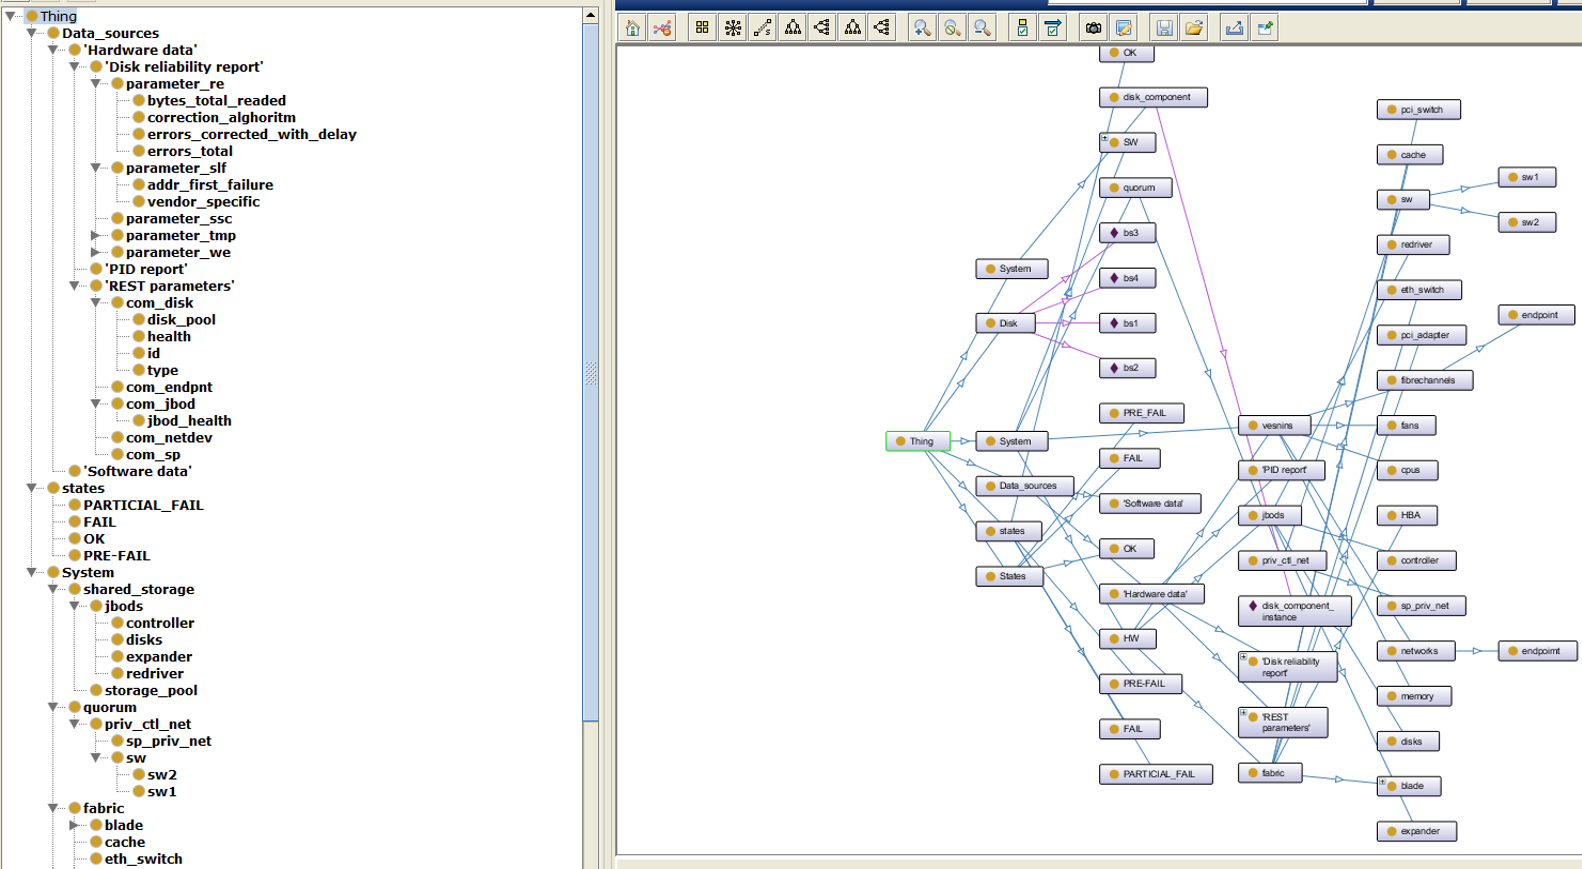
\includegraphics[width=\textwidth]{onto}
	\caption{Пример топологии системы}
	\label{fig:onto}
\end{figure}

Каждый нижележащий компонент влияет на  состояние  вышележащего  компонента,  при  этом  степень  влияния определяется кардинальностью связи consistOf. Например, для поддержания работоспособности внутренней сети (PrivateNetwork) необходимо,  чтобы входящий  в  её  состав  компонент “Виртуальный коммутатор  внутренней  сети”  (VirtualSwitch)  находился  в  работоспособном состоянии,  в  то  время  как  для  нескольких  интерфейсов  подключения контроллера  к  внутренней  сети–PrivateNetworkInterface(количество интерфейсов  равно  числу  контроллеров),  достаточно  лишь  большей  части работоспособных.

На нижнем  уровне  топологии  располагаются  элементарные компоненты  (ElementaryComponent).  Каждый  элементарный  компонент связан  только  с  одним  параметром,  на  основе  которого вычисляется состояние элементарного компонента.Таким  образом,  алгоритм  диагностирования СХД включает  в  себя решение двух подзадач:
\begin{itemize*}
	\item{оценку состояния  элементарного  компонента  на  основе  значения связанного с ним параметра;}
	\item{восстановление состояний вышележащих компонентов (в том числе системы в целом) на основе состояний нижележащих компонентов.}
\end{itemize*}
Для определения состояния компонента СХД необходимо определить все  нижележащие  компоненты,  входящие  в  состав  анализируемого компонента и вычислить их состояния.Состояние СХД в целом аналогично определяется как состояние всех компонентов СХД верхнего уровня.

Вычисление  состояния  компонентов  выполняется  при  помощи функции вычисления работоспособности компонента на основании экспертных знаний о компоненте.

На основании данного подхода предлагается методология диагностики состояний дисков????
Общая структура методологии???? представлена на рисунке ~\ref{DiagModule}.
\begin{figure}[h]
	\centering
	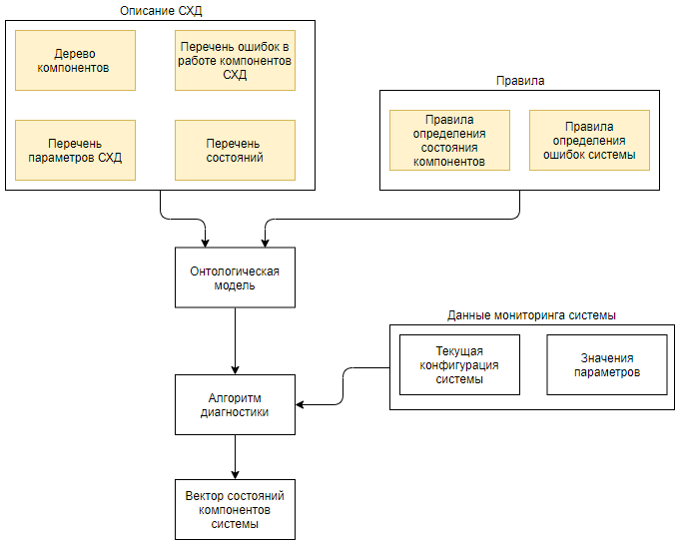
\includegraphics[width=\textwidth]{DiagModule}
	\caption{Общая схема получения параметров для модели}
	\label{fig:DiagModule}
\end{figure}

Методология построения owl модели на примере SMART параметров дисков и климатических параметров представлена на рисунке ~\ref{DataSources}.
\begin{figure}[h]
	\centering
	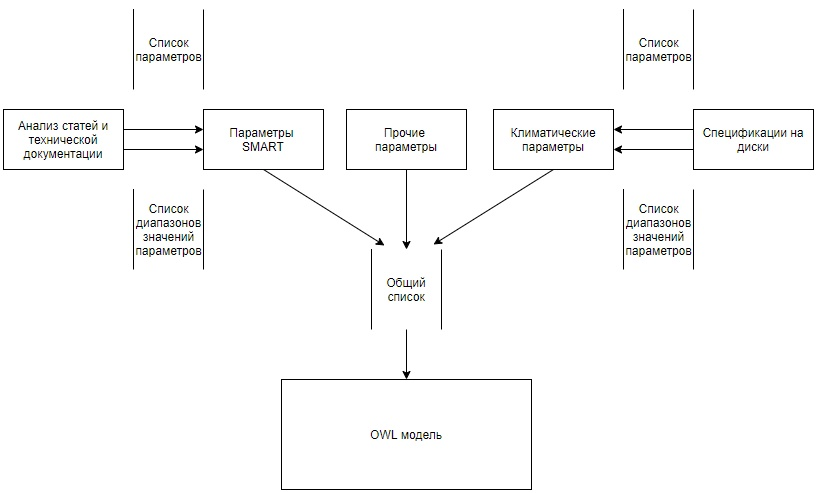
\includegraphics[width=\textwidth]{DataSources}
	\caption{Общая схема получения параметров для модели}
	\label{fig:DataSources}
\end{figure}
В главе 2 данно работы описывается исследование статей и публикаций, что в результате формирует список параметров со знчениями для наполнения owl модели. Для обеспечения полноты собираемых параметров был разработан АПК сбора климатических параметров, который обеспечивает рассматриваемую модель значениями климатических параметров. Исходя из спецификаций использууемых в СХД дисков были определены граничные значения гарантированной работы устройств. 